\chapter{Android Basics}\label{chapter:android_basics}

\section{Android Architecture}
To provide copy protection mechanisms for Android apps,
of course a deep understanding of the Android system itself
is necessary. As mentioned in~\autoref{chapter:android_status_quo},
Android is built on the Linux kernel. Android does provide not
only shell binaries (Linux kernel) but also a GUI environment
as well as predefined frameworks and a complete environment
for developers to write apps in the Java programming language.
That's why Android is considered to be a ``full software stack''
~\parencite{levin}. Although it's built on Linux,
Google did modify the Linux kernel to their need.
As a result, the Android kernel differs
incompatibly with the Linux kernel since version 2.6.27.

The difference at kernel-level is not massive compared to
the differences at user-mode where Android does have entirely new
components, namely:

\begin{itemize}
\item Dalvik Runtime including the Dalvik Virtual Machine (DVM)
respectively the Android Runtime (ART) since Android version > 5.0.
\item The Bionic C-Library instead of the GNU C Library (GlibC)
\item Hardware Abstraction Layer (HAL)
\item Java Native Interface (JNI)
\item Android specific frameworks
\end{itemize}

\autoref{fig:androidvslinux} visually summarizes the difference
between Android and Linux.

\begin{figure}[htb]
  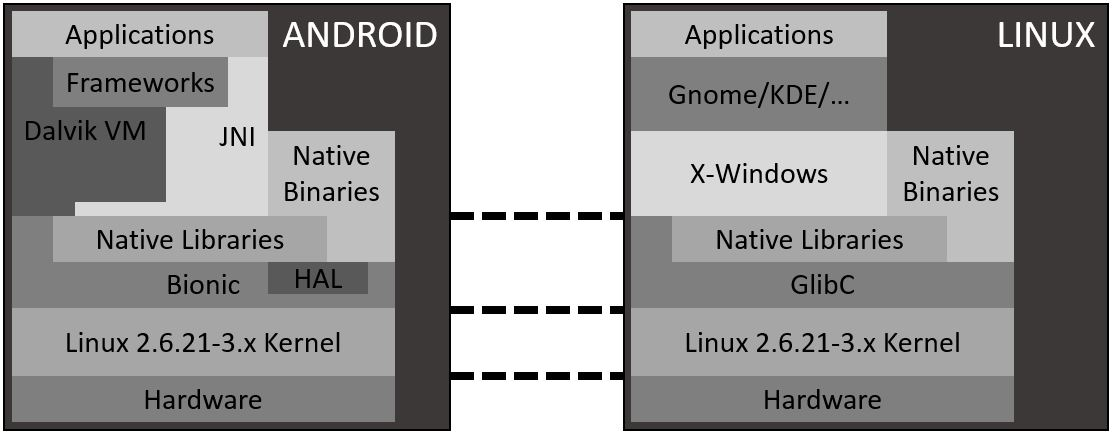
\includegraphics[width=\textwidth]{figures/androidvslinux}
  \caption[Android vs Linux]{Android and Linux comparison
  ~\parencite{levin}}
  \label{fig:androidvslinux}
\end{figure}

The Android specific frameworks are the core work that makes Android
special. They simplify the creation process of applications massively.
Developers can use the high level language Java rather than developing
in C/C++. Additionally, there is a rich set of APIs to solve most of
programmers everyday problems.

In order to get Java programs run on Android, the DVM is introduced
which is quite similar to a Java Virtual Machine (JVM).
The DVM provides an interface between the operating system and
the Java application world, after all the execution of Java programs.
The difference between DVM and JVM is the alternative form of bytecode
which gets executed in the VM. DVM is optimized for mobile devices
in terms of efficiency and sharing memory and is using the
Dalvik Executable format (DEX) as bytecode which is still device
independent ~\parencite{levin}.

With Android version 5.0, Google did introduce ART.
The prior Dalvik runtime does use Just-In-Time (JIT) compiling
where executable machine code is created not until runtime.
ART on the other hand does use Ahead-Of-Time (AOT) compilation
which compiles an app to machine code at installation time.
The reason for JIT in the first place were among other things
storage limitations of mobile devices at the time Android was released
~\parencite{levin}. As a result, the ART apps installation time
is increased as well as the required storage space as a tradeoff
to the app startup and runtime performance. As we will see,
Dalvik is still very much deep-seated in Android even under ART.

The JNI provides an opportunity to write Java programs with embedded
native processor specific code to escape from the VM world
such as direct hardware access.
It is mostly used to optimize the performance for apps (e.g games)
or to hinder reverse engineering of the application code.
Google does provide an Native Development Kit (NDK) to help
developers creating native libraries ~\parencite{ndk}.

Bionic is the Android corresponding GlibC library which was created
for license and simplicity reasons. Overall, it is more lightweight
than the GlibC and well adapted for Android.

Since Android is like to run on a great variety of devices,
it has to support a great amount of different hardware.
The HAL standardizes the interface and allows hardware vendors
to implement their own drivers ~\parencite{levin}.

\section{Android Apps}
